
\section{Cas d'utilisation : Dissémination de messages}
\label{net:sec:usecase}

La diffusion de messages d'un nœud à tous les autres est une fonctionnalité
courante des réseaux (\emph{broadcast}). La propagation épidémique
(\emph{gossip})~\cite{birman1999bimodal} constitue un moyen efficace de la
mettre en place. Sa dénomination provient de son fonctionnement : un nœud
choisit un sous-ensemble des membres du réseau et les ``contamine'' en leur
envoyant le message; les nœuds ``infectés'' en font de même; un nœud ayant déjà
envoyé le message ne le renvoie pas. Plus la taille du sous-ensemble choisi est
élevée, plus la probabilité selon laquelle le message parvient à tous les
membres du réseau augmente~\cite{erdos1959random}.

\begin{algorithm}
  
\small
\algrenewcommand{\algorithmiccomment}[1]{\hskip2em$\rhd$ #1}

\newcommand{\comment}[1]{\hfill $\rhd$ #1}

\newcommand{\LINEFOR}[2]{%
  \algorithmicfor\ {#1}\ \algorithmicdo\ {#2} %
  }

\newcommand{\LINEIFTHEN}[2]{%
  \algorithmicif\ {#1}\ \algorithmicthen\ {#2} %
  }

\newcommand{\INDSTATE}[1][1]{\State\hspace{\algorithmicindent}}

\begin{algorithmic}[1]
  \Function{broadcast}{$m$} \comment{$m$: \emph{message to send}}
  \State \textbf{let} $chosen \leftarrow getPeers(P,\, \DARKBLUE{fanout})$;
  \For{(\DARKBLUE{$n \in chosen$})}
  \State \textsc{sendTo}($n$, 'broadcast', $m$);
  \EndFor
  \EndFunction

  \Statex

  \Function{onBroadcast}{$m$} \comment{$m$: \emph{received message}}
  \If {($\DARKBLUE{\neg\textsc{alreadyReceived}(m)}$)}
  \State \textsc{broadcast}($m$);
  \EndIf
  \EndFunction
\end{algorithmic}

  \caption[Algorithme de dissémination de
  messages]{\label{net:algo:broadcast}Algorithme de dissémination de messages.}
\end{algorithm}


L'algorithme~\ref{net:algo:broadcast} montre les quelques instructions composant
la dissémination épidémique de messages. L'épanouissement (\emph{fanout})
désigne le nombre de voisins auxquels le message va être envoyé. La fonction
\textsc{getPeers} renvoie autant de nœuds distincts. Dans le cadre d'approches
fournissant une vue partielle de taille constante, cette variable
d'épanouissement est elle aussi constante, et configurée à l'avance. Pour que
les chemins employés lors de la dissémination soient eux aussi aléatoires malgré
la fréquence beaucoup plus faible des échanges du protocole d'échantillonnage,
la taille de la vue est nettement surestimée~\cite{frey2009heterogeneous}. Par
exemple, une vue partielle contient 30 arcs, mais seulement 6 sont employés à
chaque dissémination. Dans le cadre de \SPRAY, nous augmentons les tailles des
vues partielles fournies : lors de l'entrée dans le réseau, un nœud n'ajoute
plus qu'une seule référence au contact mais $c$ doublons; les vues partielles
tendent vers $c\cdot\ln(|\mathcal{N}|)$~\cite{ganesh2003peer}; un nœud détectant
un départ ou une panne ajuste la probabilité de supprimer un arc à
$c \div (|P|+occ)$. La variable d'épanouissement est configurée comme étant une
fraction de la vue partielle. Ainsi l'épanouissement peut s'ajuster
automatiquement pour suivre une progression logarithmique :
$\ln(|\mathcal{N}|)+x$, où $x$ est un entier positif.

La suite met en évidence l'avantage apporté par une variable d'épanouissement
s'ajustant à la taille du réseau. En particulier, nous mesurerons le taux de
réception totale des messages par les membres du réseau. Si au moins un membre
ne reçoit pas le message, alors la réception totale à échouée. Le taux mesuré
est le nombre de messages ayant été reçus par tout les membres sur le nombre de
messages ayant été envoyés.

\paragraph{Objectif :} Montrer les bénéfices apportées au mécanisme de
dissémination par un protocole adaptatif d'échantillonnage.

\paragraph{Description :} L'application considérée cible approximativement 100
nœuds. Les vues partielles fournies par \CYCLON sont configurées pour contenir
30 voisins ($6 \cdot \ln(100) \approx 6 \cdot 5 = 30$). Nous considérons 2
configurations pour l'épanouissement : $\ln(100)+1 \approx 6$ et
$\ln(100)+3 \approx 8$. Ces configurations garantissent une forte probabilité de
réception des messages lorsque le réseau contient 100 nœuds ou moins. De même,
nous configurons \SPRAY pour qu'il fournisse des vues partielles 6 fois plus
peuplés qu'à la normale. La variable d'épanouissement est configurée pour
choisir 1 sixième de la vue, soit $\ln(|\mathcal{N}|)+1$ et
$\ln(|\mathcal{N}|)+3$.  Les deux protocoles d'échantillonnage aléatoire
possèdent donc les même configurations pour un réseau de 100 nœuds. La taille
des réseaux considérés grandit de 0.1k à 2k nœuds. Nous mesurons à chaque cycle
la fraction, sur 1k messages, parvenant à l'intégralité des membres du réseau.

\begin{figure}
  \begin{center}
    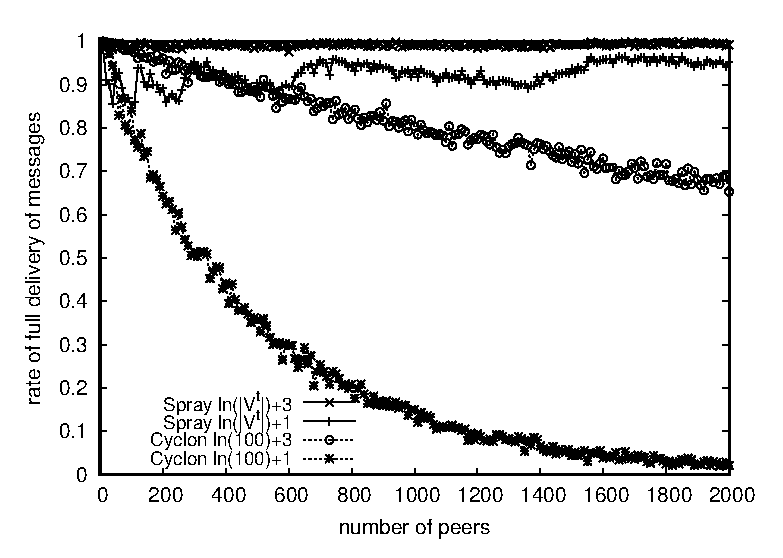
\includegraphics[width=.8\textwidth]{img/spray/hardrate.eps}
    \caption[Taux de réception des messages comparé à la taille du
    réseau.]{\label{net:fig:hardrate} Taux de réception des messages comparé à
      la taille du réseau. L'axe des abscisses montre la taille du réseau en
      nombre de nœuds. L'axe des ordonnées montre le taux de réception total
      mesuré sur 1k messages.}
  \end{center}
\end{figure}

\paragraph{Résultat :} La figure~\ref{net:fig:hardrate} présente les résultats
de cette simulation. Tout d'abord, nous observons que le taux de réception des
messages avec \CYCLON souffre d'une constante décroissance. De moins en moins de
messages parviennent à l'ensemble des nœuds lorsque le réseau s'agrandit. La
configuration dont la variable d'épanouissement est la plus élevée fournie de
meilleurs résultats. En revanche, le taux de réception des messages de \SPRAY
reste stable bien que nous puissions observer la présence de petits sauts dans
les valeurs mesurées. Un épanouissement initialisé à $\ln(|\mathcal{N}|)+1$
conduit à un taux aux environs de 90\%. Un épanouissement initialisé à
$\ln(|\mathcal{N}|)+3$ conduit à un taux proche de 100\%. Globalement, le
mécanisme de dissémination épidémique présenté profite bien de la nature
adaptative de \SPRAY. Cela lui permet de s'ajuster aux besoins d'un réseau dont
la taille fluctue au cours du temps.

\paragraph{Explication :} Le seuil précis de connexité d'un graphe aléatoire est
$\Theta(|\mathcal{N}|\ln(|\mathcal{N}|))$ arcs. Pour la dissémination de
messages cela signifie que, avec des vues partielles suffisamment grandes et
peuplées d'arcs vers des nœuds suffisamment aléatoires, un épanouissement fixé à
$\ln(|\mathcal{N}|)$ conduit à un taux de réception aux environs de 50\%. À ce
stade, incrémenter cette variable augmente drastiquement le taux de
réception. Cependant, la contribution de chaque incrémentation diminue petit à
petit par rapport à l'incrémentation précédente. Le mécanisme de dissémination
construit au dessus de \CYCLON possède un épanouissement constant, configuré
pour une taille spécifique du réseau. Tant que la taille du réseau est
inférieure ou égale à la taille ciblée, le taux de réception demeure élevé. En
revanche, une fois cette taille dépassée, le taux de réception chute très
rapidement. \SPRAY donne la possibilité au mécanisme de dissémination d'ajuster
sa variable d'épanouissement à la taille du réseau. Ainsi, le taux de réception
des messages reste stable, même lorsque le réseau s'agrandit. Les petits sauts
mesurées sont dûs au fait que les valeurs manipulées localement par chaque nœuds
sont des entiers. Le bond correspond donc à une valeur arrondie augmentant
suffisamment pour être incrémentée.

%%%%%%

\paragraph{Objectif :} Montrer comment le taux de réception des messages se
comporte lors d'un pique de population, i.e., une augmentation massive de la
taille du réseau suivie peut après d'une diminution.

\paragraph{Description :} Nous configurons \SPRAY et \CYCLON de la même manière
que pour la précédente simulation. Pour \CYCLON, les vues partielles sont
initialisées à 30 voisins avec deux valeurs pour l'épanouissement : $\ln(100)+1$
et $\ln(100)+3$. Pour \SPRAY, les vues partielles s'ajustent automatiquement à
$6\cdot \ln(|\mathcal{N}|)$ et les valeurs d'épanouissement s'ajustent
automatiquement à $\ln(|\mathcal{N}|)+1$ et $\ln(|\mathcal{N}|)+3$. La
simulation commence avec 0.1k nœuds. Le réseau atteint rapidement 10k nœuds
pendant le pique de popularité. Enfin il redescend à 3k nœuds. Dans cette
simulation, nous mesurons le taux de réception total des messages sur 0.1k
messages.

\begin{figure}
  \begin{center}
    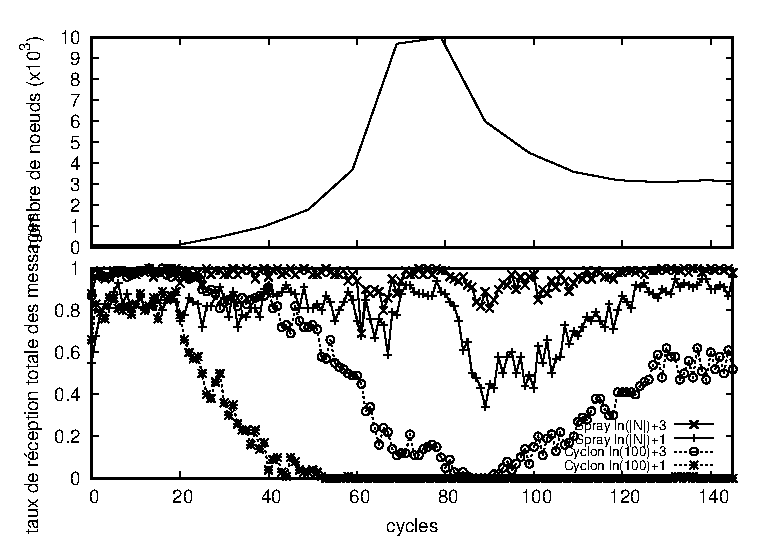
\includegraphics[width=.8\textwidth]{img/spray/peak.eps}
    \caption[Taux de réception des messages lors d'un pique de
    population]{\label{net:fig:peak} Taux de réception des messages lors d'un
      pique d'entrée dans le réseau. L'axe des abscisses montre le temps en
      nombre de cycles. L'axe des ordonnées de la partie haute montre le nombre
      de nœuds présent dans le réseau. L'axe des ordonnées de la partie basse
      montre le taux de réception des messages sur 0.1k messages.}
  \end{center}
\end{figure}

\paragraph{Résultat :} La figure~\ref{net:fig:peak} montre les résultats de
cette simulation. Tout comme lors de la simulation précédente, l'utilisation de
\CYCLON et d'une variable d'épanouissement prédéfinie fonctionne jusqu'à ce que
la taille du réseau excède la taille prévue. Pendant le pique d'entrée dans le
réseau, le taux de réception chute très rapidement. À l'inverse, le mécanisme de
dissémination construit avec \LSEQ ajuste automatiquement sa variable
d'épanouissement à la taille du réseau. Ainsi, le système ne souffre pas de
sévère baisse du taux de réception lors du pique d'entrée. Cependant, lors du
départ massif de certains membres, le taux de réception chute. Cela est
particulièrement vrai pour la configuration de \SPRAY avec un épanouissement
plus modeste de $\ln(|\mathcal{N}|)+1$. Globalement, le mécanisme de
dissémination se comporte mieux avec \SPRAY et devient résilient aux
fluctuations rapides de la taille des réseaux.

\paragraph{Explication :} La variable d'épanouissement des configurations
impliquant \CYCLON est constante. Ainsi, lorsque la taille du réseau dépasse la
taille prévue, le taux de réception chute drastiquement. À l'opposé, la
variable d'épanouissement des configurations basés sur \SPRAY suit les
évolutions du réseau. Le taux de réception reste stable lors d'augmentations
rapides de la taille du réseau. Cependant, à la fois \CYCLON et \SPRAY détectent
les nœuds partis lors de la phase d'échange de vues partielles. Les arcs
obsolètes sont malgré tout utilisés dans la dissémination. Par conséquent, un
plus grand nombre de messages à tendance à se perdre. Petit à petit, les arcs
obsolètes disparaissent des vues partielles. Le taux de réception des messages
recouvre sa valeur attendue.

%%% Local Variables:
%%% mode: latex
%%% TeX-master: "../../paper"
%%% End:
